\begin{figure}[htbp]
\centering
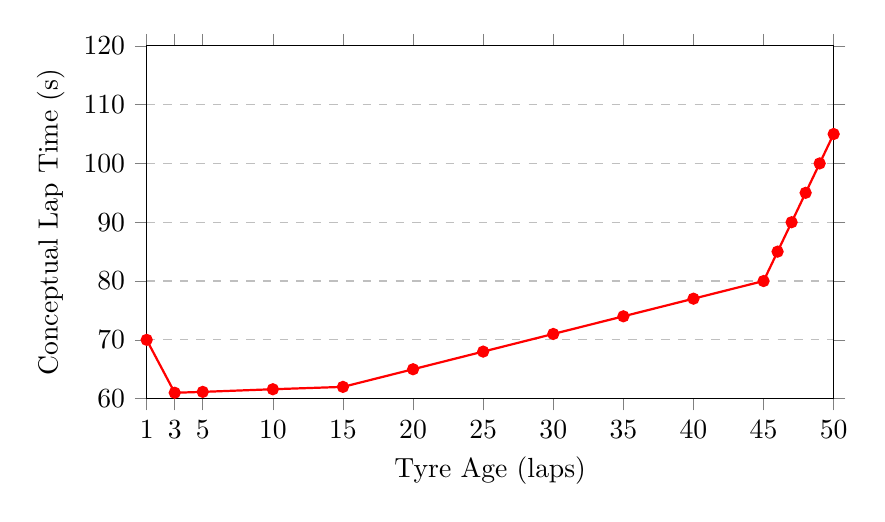
\begin{tikzpicture}
\begin{axis}[
    width=0.85\textwidth,
    height=0.5\textwidth,
    xlabel={Tyre Age (laps)},
    ylabel={Conceptual Lap Time (s)},
    xmin=1,
    xmax=50,
    ymin=60,
    ymax=120,
    ytick={60,70,80,90,100,110,120},
    xtick={1,3,5,10,15,20,25,30,35,40,45,50},
    ymajorgrids=true,
    grid style=dashed,
    legend style={
        at={(0.5,1.02)},
        anchor=south,
        legend columns=3,
        draw=none
    },
    tick align=outside
]

% Soft
\addplot[
    thick,
    red,
    mark=*,
    mark size=1.8pt
] coordinates {
(1,70)
(3,61)
(5,61.15)
(10,61.6)
(15,62)
(20,65)
(25,68)
(30,71)
(35,74)
(40,77)
(45,80)
(46,85)
(47,90)
(48,95)
(49,100)
(50,105)
};

\end{axis}
\end{tikzpicture}
\caption{Conceptual tyre degradation model of tyre lifecycle, demonstrating the four distinct phases of tyre behaviour - ramping up (laps 1-3), peak grip (laps 3-15), degradation (laps 15-45), and the cliff (laps 45-50).}
\label{fig:1_tyre_life}
\end{figure}